\documentclass[11pt, oneside]{article} 
\usepackage{geometry}
\geometry{letterpaper} 
\usepackage{graphicx}
	
\usepackage{amssymb}
\usepackage{amsmath}
\usepackage{parskip}
\usepackage{color}
\usepackage{hyperref}

\graphicspath{{/Users/telliott/Github/precalculus/fig/}}
% \begin{center} \includegraphics [scale=0.4] {gauss3.png} \end{center}

\title{Perpendicular bisector}
\date{}

\begin{document}
\maketitle
\Large

\subsection*{perpendicular at a point}

We often will wish to construct a line or line segment perpendicular to another line segment.  This may be specified to occur at a particular (given) point, either on the line, or not on the line.  

For the first case, consider the horizontal line below (left panel) and suppose we know a point on the line $P$ and wish to construct the vertical line through $P$.  The procedure is to use the compass to mark off points $Q$ and $R$ on the line an equal distance from $P$.  

This can be done by drawing a circle with center at $P$.

\begin{center} 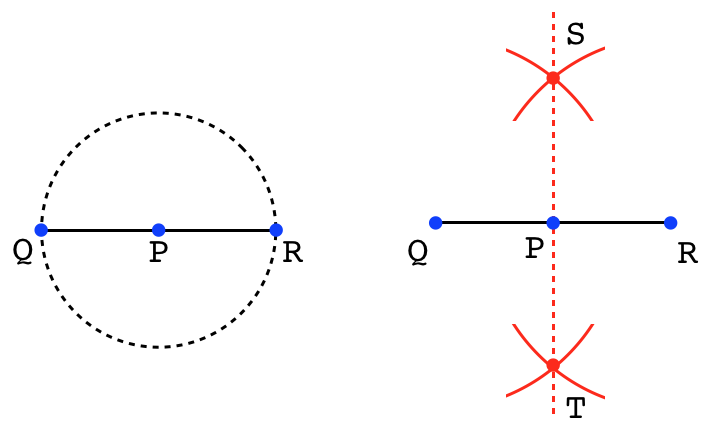
\includegraphics [scale=0.4] {perp_1.png} \end{center}

Using the compass again (right panel), find $S$ equally distant from $Q$ and $R$ ($QS = RS$).  This can be done by using the compass to draw slightly larger circles of the same radius on centers $Q$ and $R$.

 The line segment $SP$ will be perpendicular to the line containing $QPR$.

There is a restriction in Euclid's Elements to a collapsible compass, one which loses its setting when lifted from the page.  

That might make it impossible to find $S$ as just stated.  However, one can simply draw a circle of radius exactly equal to $QR$ centered at $Q$ and another one with the same radius, centered at $R$.

\subsection*{bisect a line segment}

Suppose that we had not known the point $P$ when we started the procedure above, but already had two points $Q$ and $R$.

Then the line through $S$ and $T$ crosses $QR$ at its midpoint, and we have found the point $P$ that bisects $QR$.

\subsection*{perpendicular through a point}

Alternatively, suppose we know the line and the point $S$ but not $P$, and we wish to construct a vertical through the line that also passes through $S$.  Find $Q$ and $R$ on the line an equal distance from $S$ ($QS$ = $RS$), as radii of a circle centered at $S$ (left panel, below).  Their exact position is unimportant.  

\begin{center} 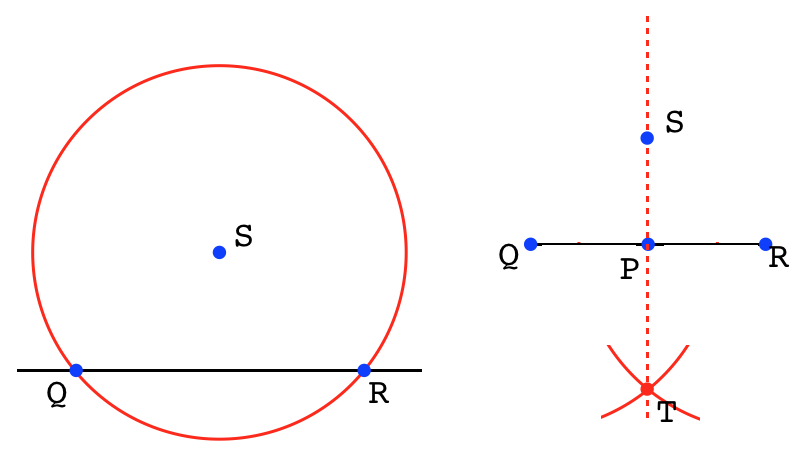
\includegraphics [scale=0.35] {perp_2.png} \end{center}

Also find $T$ such that $QT = RT$, using circles with radius $QR$ centered at $Q$ and $R$, as before.  

The line segment $ST$ is perpendicular to the line segment containing $QR$, and passes through $S$, as required.

Also, see the video at the url:

\url{https://www.mathopenref.com/constperpextpoint.html}

\subsection*{bisector properties}

Using what we've just learned, suppose we know two points $Q$ and $R$.  We find the point $P$ equidistant between them and construct the perpendicular bisector $PS$.  Then the two sides $SQ$ and $SR$ have equal length.  Triangle $\triangle SQR$ is isosceles.

\begin{center} 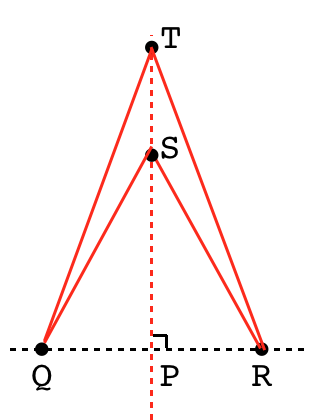
\includegraphics [scale=0.45] {perp_3.png} \end{center}

Proof.

By construction, $PQ = PR$, $\angle SPR$ is a right angle, and side $SP$ is shared.  Hence the two triangles $\triangle SPQ$ and $\triangle SPR$ are congruent, by SAS.

$\square$

This is true for \emph{any} point on the line drawn through $S$ and $P$.  For example, $TQ = TR$ in the figure above.

\subsection*{three points}

Now, suppose we have three points:  $Q$, $R$ and $S$.  We find the perpendicular bisector of $QR$ and also, the perpendicular bisector of $QS$.  Extend them to where they meet, at point $O$.

\begin{center} 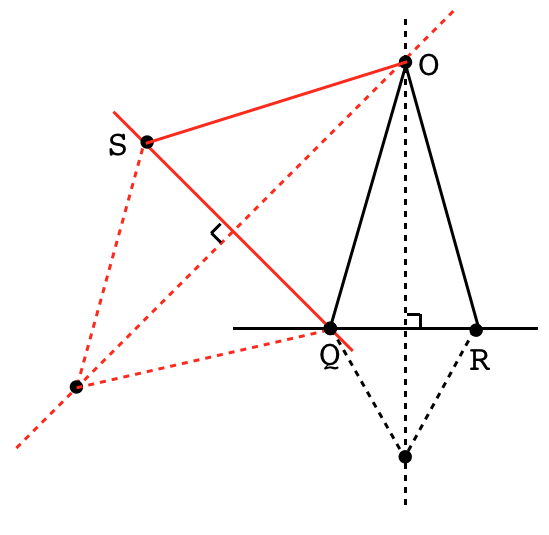
\includegraphics [scale=0.35] {perp_4.png} \end{center}

What can we say about point $O$?

$\circ$ \ $O$ is equidistant from $Q$ and $R$.

$\circ$ \ $O$ is also equidistant from $Q$ and $S$.

Therefore, $OQ = OR = OS$.  If we draw a circle on center $O$, it will pass through all three points.

\begin{center} 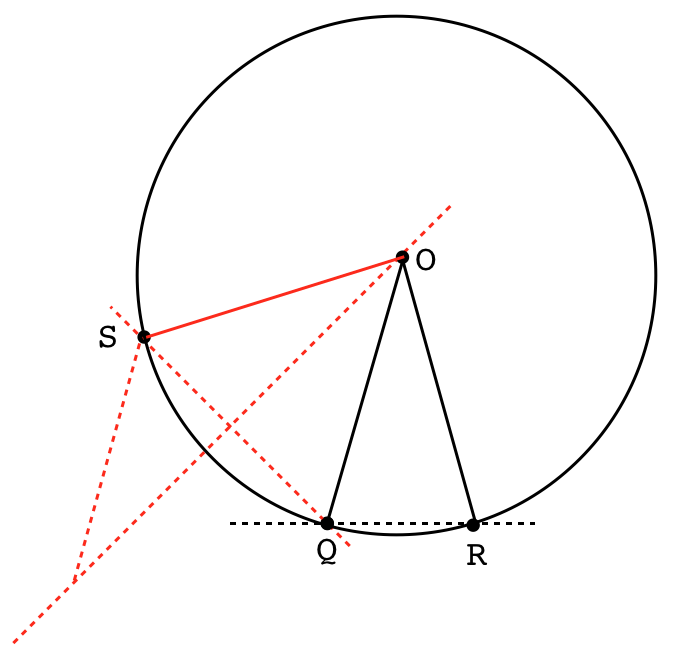
\includegraphics [scale=0.3] {perp_5.png} \end{center}

\subsection*{circumcenter}

The point where the perpendicular bisectors cross has a special name, it is called the circumcenter.

\begin{center} 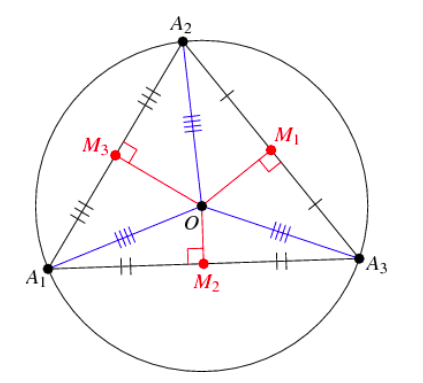
\includegraphics [scale=0.5] {three_point_circle2.png} \end{center}

There are other special points where interesting circles can be drawn.

\end{document}